% ============================ PHASE 2 ==================================
\newpage
\phase{Phase two \textbullet\ The problem and the promise}{Today's hydrogen is dirty, and India pays for it twice}{How hydrogen is made now, what that costs the climate and the exchequer, what ``green'' really promises, and the goals it serves.}

\subsection{How the world makes hydrogen today}

The world used almost 100 million tonnes of hydrogen in 2024, and the vast majority came from fossil fuels with no carbon capture at all \cite{ieanews2025}. In 2023 nearly two-thirds was made from natural gas and about a fifth from coal \cite{ieaghr2024}. \confH

The usual method is \emph{steam methane reforming}. In plain words: you heat natural gas with steam until the molecules break apart, keep the hydrogen, and release the carbon as \coo. The International Energy Agency (IEA) puts the damage at \textbf{10–12 kg of \coo-equivalent for every kilogram of hydrogen made from gas, and 22–26 kg when it is made from coal} \cite{ieaghr2024}.

\begin{figure}[H]
\centering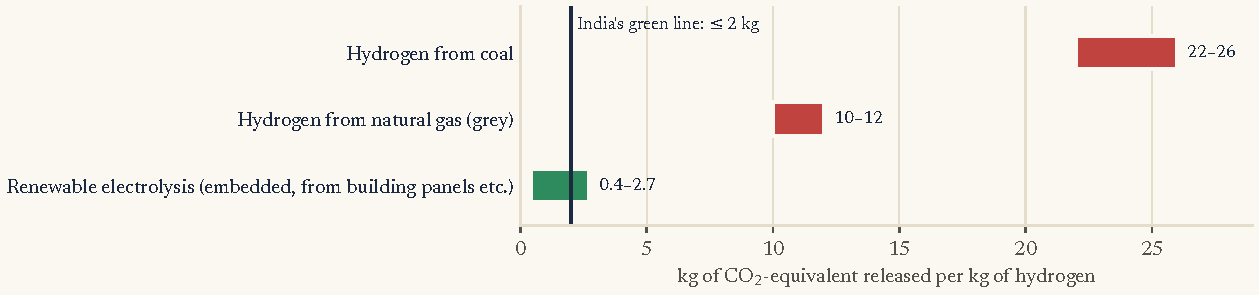
\includegraphics[width=0.98\textwidth]{figures/emissions.pdf}
\caption{Carbon released per kilogram of hydrogen, by production route. Data: \cite{ieaghr2024}; India's threshold: \cite{drishti2023}.}
\end{figure}

Add it up and hydrogen production released about \textbf{920 million tonnes of \coo{} in 2023} \cite{ieaghr2024}. Against the 37.4 billion tonnes of energy-related \coo{} the world emitted that year \cite{ieaco2}, that is roughly 2.5\%, more than most countries emit in total. Ammonia alone accounts for about 450 million tonnes of direct emissions a year, roughly 2.4 tonnes of \coo{} per tonne made, which the IEA notes equals the whole energy system of South Africa \cite{ieaammonia2021}. \confH

\subsection{The double bill India pays}

\begin{center}
\begin{tikzpicture}[
  col/.style={rounded corners=2pt,fill=wash,text width=68mm,minimum height=50mm,anchor=north west,inner sep=7pt,align=left}]
\node[col] (a) at (0,0) {%
  {\eyebrowfont\fontsize{6.6}{8}\selectfont\color{audit}BILL ONE \textbullet\ THE CARBON BILL}\\[5pt]
  {\display\fontsize{20}{22}\selectfont\color{ink}55–70 Mt}\\[2pt]
  {\footnotesize of \coo{} a year from the hydrogen India makes at home. My arithmetic: about 5.6 Mt of grey hydrogen \cite{igef2021} $\times$ 10–12 kg \coo{} per kg \cite{ieaghr2024}. The Mission's own target of 50 Mt avoided for 5 Mt of green hydrogen implies the same ratio \cite{govnow2023}.}};
\node[col] (b) at (76mm,0) {%
  {\eyebrowfont\fontsize{6.6}{8}\selectfont\color{audit}BILL TWO \textbullet\ THE DOLLAR BILL}\\[5pt]
  {\display\fontsize{20}{22}\selectfont\color{ink}₹1.86 lakh crore}\\[2pt]
  {\footnotesize fertiliser subsidy in FY26 (revised), with urea alone at ₹1.26 lakh crore \cite{skfert2026}. Roughly half of India's gas is imported \cite{etv2025,kpmg2026}, and the fertiliser sector takes 58\% of the imported LNG India regasifies \cite{kpmg2026}. Urea imports may have topped 10 Mt in FY26 \cite{skfert2026}.}};
\end{tikzpicture}
\end{center}
{\small\itshape\color{ink2} Confidence in both bills: \confM\ (the carbon figure is my arithmetic on 2018–19 volumes; the subsidy figure comes from a news digest of the Union Budget).}

Here is the part that took me a while to see. The farmer does not feel a gas-price shock, because the retail price of urea has been frozen at ₹5,360 a tonne since November 2012 \cite{skfert2026}. \textbf{The government absorbs the shock instead.} When the rupee slid from about 86.6 to 91.9 to the dollar, the subsidy bill rose with it \cite{skfert2026}. So the real owner of India's grey-hydrogen risk is the exchequer.

\begin{finding}[Key finding \textbullet\ green hydrogen is a hedge before it is a climate tool]
Grey hydrogen's cost moves with imported gas and the rupee. Green hydrogen's cost is mostly capital, fixed on the day the plant is financed. When SECI signs a 10-year fixed-price green-ammonia contract \cite{pvm2025}, the state is really buying an \emph{insurance policy}: it swaps a volatile, dollar-linked cost for a known rupee number. For a finance student this is the cleanest way to explain why a ``more expensive'' molecule can still be the cheaper choice. \confH\ on the mechanism, \confM\ on its size.
\end{finding}

\subsection{What ``green'' actually promises}

India wrote its definition down in August 2023. Hydrogen counts as \textbf{green} only if it is made from renewable energy, by electrolysis or by converting biomass, and emits \textbf{no more than 2 kg of \coo-equivalent per kg of hydrogen}. That is measured ``well-to-gate'', covering water treatment, electrolysis, purification, drying and compression, and averaged over the previous 12 months. The Bureau of Energy Efficiency accredits the agencies that check it \cite{drishti2023}. \confH

\begin{table}[tbp]\centering\tablefont
\caption{The hydrogen ``colours'' that matter for an Indian decision.}
\begin{tabularx}{\textwidth}{@{}p{21mm} L p{25mm} L l@{}}
\toprule
\thead{Colour} & \thead{How it is made} & \thead{\coo{} per kg H\textsubscript{2}} & \thead{Cost and status in India} & \thead{Conf.}\\ \midrule
\textbf{Grey} & Natural gas split with steam, carbon vented & 10–12 kg \cite{ieaghr2024} & About \usd{}2.1–2.2/kg \cite{jmkiocl2025,tribune2025}. The default today. & \confH\\
\textbf{Black/brown} & Coal gasified, carbon vented & 22–26 kg \cite{ieaghr2024} & Minor in India; the dirtiest route. & \confH\\
\textbf{Blue} & Grey plus carbon capture and storage & Lower, depends on capture rate and methane leaks & Capture costs \usd{}60–110 per tonne of \coo{} \cite{ieaghr2024}, adding roughly \usd{}0.3–1.2/kg at 55–90\% capture (my arithmetic). I found no large Indian CO\textsubscript{2} storage hub to send it to. & \confL\\
\textbf{Green} \newline (electrolysis) & Water split with renewable power & $\le$2 kg by law \cite{drishti2023} & \usd{}3.5–4/kg today \cite{tribune2025}; refinery contracts at ₹279–397/kg \cite{rwnrl2026,jmkiocl2025}. & \confH\\
\textbf{Green} \newline (biomass) & Crop waste or biogas converted to hydrogen & Counts as green under India's standard \cite{drishti2023} & Early pilots; limited by collecting enough feedstock. & \confL\\
\bottomrule
\end{tabularx}
\end{table}

Three honest caveats keep the promise from becoming a slogan.

\begin{itemize}
\item \textbf{Building the panels has a footprint.} Manufacturing the renewable plant embeds 0.4–2.7 kg \coo{} per kg of hydrogen, which most standards do not count \cite{ieaghr2024}. \confH
\item \textbf{Leaks warm the planet.} A multi-model study put hydrogen's 100-year global warming potential at about 11.6 times that of \coo{} \cite{sand2023}. Hydrogen does not trap heat directly, but in the air it lengthens the life of methane and other warming gases. A leaky green plant is less green than it looks. \confM
\item \textbf{Water is a smaller problem than people fear, but location matters.} Green hydrogen uses about 20–30 litres per kg once purification and cooling are counted, on par with or below grey hydrogen's 20–40 litres \cite{rmi2023}. The issue is not the total but \emph{which district} the water comes from. Coastal sites with desalination avoid the fight. \confH
\end{itemize}

\subsection{The goals it serves}

\begin{figure}[H]
\centering
\begin{tikzpicture}[x=1mm,y=1mm,
  milestone/.style={circle,fill=#1,minimum size=4mm,inner sep=0},
  txt/.style={anchor=north,text width=34mm,align=center,font=\footnotesize}]
\draw[rule,line width=2pt] (0,0) -- (150,0);
\foreach \x/\yr/\c/\body in {
 4/2015/ink2/{\textbf{Paris Agreement}: hold warming well below 2\,°C, aim for 1.5\,°C \cite{paris}},
 42/2023/brass/{\textbf{Mission launched}: ₹19,744 crore, 5 Mt of green hydrogen a year by 2030 \cite{govnow2023}},
 80/2025/sgreen/{\textbf{50\% non-fossil power capacity} reached, five years early: 242.8 of 484.8 GW \cite{energetica2025}},
 112/2030/sblue/{\textbf{NDC}: 45\% lower emissions intensity of GDP than 2005 \cite{powerline2022}},
 146/2070/audit/{\textbf{Net zero} for India \cite{powerline2022}}}{
 \node[milestone=\c] at (\x,0) {};
 \node[font=\display\fontsize{11}{12}\selectfont,text=\c,anchor=south] at (\x,3) {\yr};
 \node[txt] at (\x,-4) {\body};
}
\end{tikzpicture}
\caption{The commitments green hydrogen is meant to serve.}
\end{figure}

The National Green Hydrogen Mission is the bridge between these targets and our plant. Its promised 2030 outcomes are worth quoting exactly, because every one of them is a stakeholder interest we will meet again in the project: \textbf{at least 5 million tonnes a year of green hydrogen, about 125 GW of new renewable capacity, over ₹8 lakh crore of investment, over 6 lakh jobs, over ₹1 lakh crore of cumulative fossil-fuel import savings, and about 50 million tonnes a year of greenhouse gas avoided} \cite{govnow2023}. Of the ₹19,744 crore outlay, ₹17,490 crore sits in SIGHT, the incentive scheme that funds electrolyser factories and green hydrogen and ammonia production \cite{govnow2023}. \confH

Two more goals give the case teeth. First, the UN Sustainable Development Goals: green hydrogen speaks directly to clean energy (SDG 7), industry and infrastructure (SDG 9) and climate action (SDG 13), and through fertiliser security to zero hunger (SDG 2) \cite{unsdg}. Second, Europe's border carbon charge. The definitive phase of the EU's Carbon Border Adjustment Mechanism began in January 2026 and covers both hydrogen and fertilisers, including ammonia \cite{coolset}. Any Indian exporter of grey ammonia to Europe will eventually pay for its carbon; a green exporter will not. \confH

\subsection{Promise versus delivery}

Ambition is cheap. Here is the scoreboard as of 2026.

\begin{center}
\begin{tikzpicture}[x=1mm,y=1mm]
\foreach \x/\bg/\sm/\cc in {
 0/{862,000 t}/{a year of green hydrogen capacity allocated to 19 companies \cite{rw2025}}/ink,
 52/{$\approx$8,000 t}/{a year actually commissioned by February 2026 \cite{chemindigest2026}, under 1\% of the allocation}/audit,
 104/{$\approx$9\%}/{utilisation of the world's 58 GW a year of electrolyser factories in 2025 \cite{argus2026}}/brass}{
\fill[wash,rounded corners=2pt] (\x,0) rectangle (\x+48,30);
\node[anchor=north west,font=\display\fontsize{17}{19}\selectfont,text=\cc] at (\x+3,27) {\bg};
\node[anchor=north west,text width=42mm,font=\footnotesize] at (\x+3,16) {\sm};
}
\end{tikzpicture}
\end{center}

Globally, 2025 was a correction. Developers committed to roughly 1 million tonnes a year of new low-emission capacity but cancelled over 4.9 million tonnes' worth \cite{chemworld2026}. The IEA cut its estimate of 2030 low-emission output from 49 to 37 million tonnes a year \cite{ieanews2025}. Oman's \usd{}6.7 billion HyDuqm project was dropped after its partners reviewed ``offtake dynamics'', which is polite language for ``nobody signed to buy'' \cite{meed2025}. \confH

\begin{verdict}[My verdict on ``future-proof and necessary'']
\emph{Necessary}: yes, for the fertiliser, refining, steel and shipping jobs that nothing else can do, and because it turns an imported, volatile cost into a domestic, fixed one. \emph{Future-proof}: only conditionally. The projects that survived 2025 had one thing in common, a creditworthy buyer under a long contract. Green hydrogen is a future-proof idea; any single green hydrogen plant is only as future-proof as its offtake contract. That sentence becomes the first rule of our project. \confH
\end{verdict}
